\section{Introduction}

\begin{frame}\frametitle{Types of documents}

\begin{itemize}
\item
  Types

  \begin{itemize}
  \item
    Journal articles, books, book chapters, theses
  \item
    Preliminary analyses
  \item
    Online content: web pages, blog posts, forum posts
  \item
    Slide show presentations
  \item
    Consulting reports
  \end{itemize}
\item
  Key Distinctions

  \begin{itemize}
  \item
    online versus paper-based
  \item
    document or presentation
  \item
    audience: formal versus informal (e.g., self, collaborators)
  \end{itemize}
\end{itemize}

\end{frame}

\begin{frame}\frametitle{What is \emph{reproducible analysis}?}

\begin{itemize}
\item
  Reproducibility varies on a continuum
\item
  I operationalise it as:

  \begin{itemize}
  \item
    code transforms raw data and meta-data into processed data,
  \item
    code runs analyses on the data, and
  \item
    code incorporates analyses into a report
  \end{itemize}
\item
  Ideally, the process has a one-click build
\item
  Public sharing of document, code, and data is optional, but forms part
  of gold standard of scientific openness
\item
  Goes by many names, particularly ``reproducible research'', but I
  prefer ``reproducible analysis''.
\end{itemize}

\tiny{
See also: \url{http://stats.stackexchange.com/a/15006/183} 
\url{https://github.com/jeromyanglim/rmarkdown-rmeetup-2012/issues/11}}

\end{frame}

\begin{frame}\frametitle{Aims of Reproducible}

\begin{itemize}
\item
  Ability to reproduce analysis
\item
  Increase accuracy

  \begin{itemize}
  \item
    Ability to verify analyses are consistent with intentions
  \item
    Ability to review analysis choices
  \end{itemize}
\item
  Increase clarity of communication
\item
  Increased trustworthiness

  \begin{itemize}
  \item
    Increased accuracy +
  \item
    Ability for others to verify
  \end{itemize}
\item
  Extensibility

  \begin{itemize}
  \item
    Ability to easily modify or re-use existing analyses
  \end{itemize}
\end{itemize}

\end{frame}

\section{Markdown}

\begin{frame}\frametitle{Overview of Markdown}

\begin{itemize}
\item
  Ultra simplified and intuitive set of markup
\item
  Limited set of markup
\item
  HTML passed straight through
\item
  Various extensions
\item
  Popular on websites: e.g., StackOverflow, GitHub, Reddit
\end{itemize}

\end{frame}

\begin{frame}\frametitle{Headings}

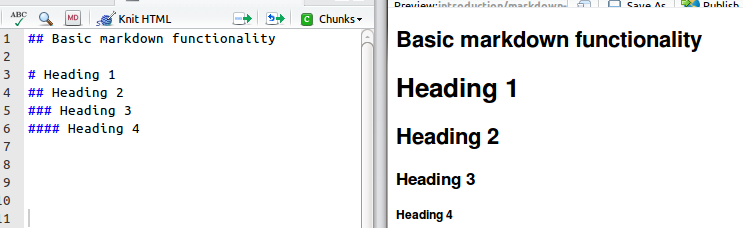
\includegraphics[width=4in]{figures/headings.png}

\end{frame}

\begin{frame}\frametitle{Basic formatting}

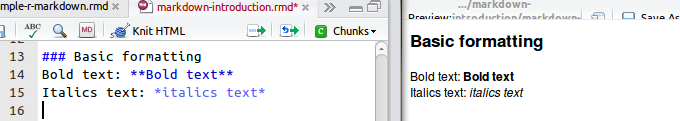
\includegraphics[width=4in]{figures/basic-formatting.png}

\end{frame}

\begin{frame}\frametitle{Paragraphs}

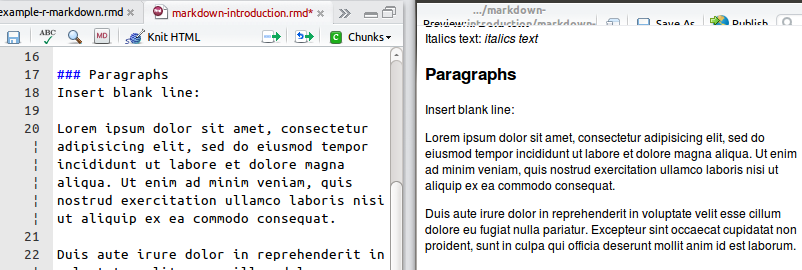
\includegraphics[width=4in]{figures/paragraphs.png}

\end{frame}

\begin{frame}\frametitle{Dot points}

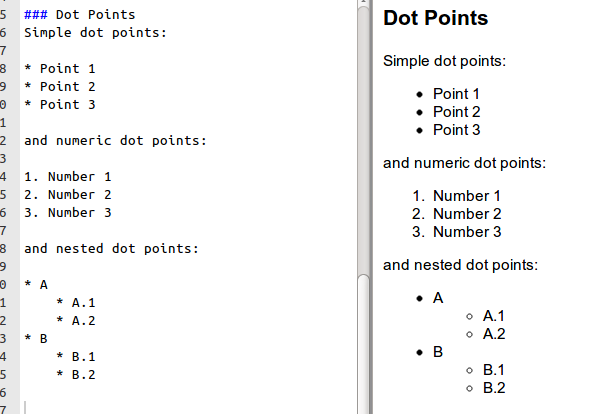
\includegraphics[width=4in]{figures/dot-points.png}

\end{frame}

\begin{frame}\frametitle{Equations}

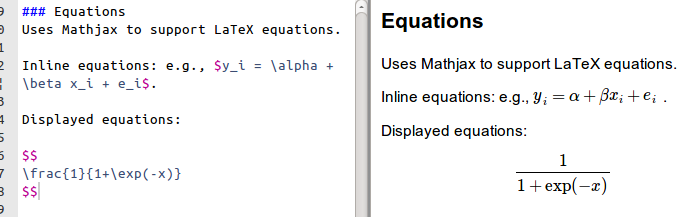
\includegraphics[width=4in]{figures/equations.png}

\end{frame}

\begin{frame}\frametitle{Hyperlinks}


\includegraphics[width=4in]{figures/links.png}

\end{frame}

\begin{frame}\frametitle{Images}

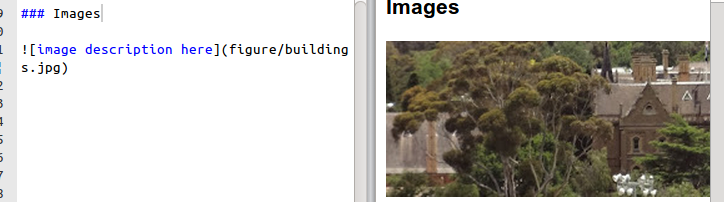
\includegraphics[width=4in]{figures/images.png}

\end{frame}

\begin{frame}\frametitle{Code}

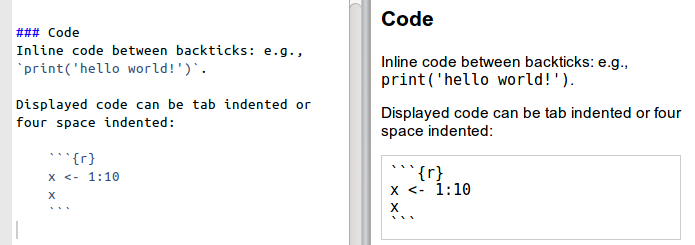
\includegraphics[width=4in]{figures/code.png}

\end{frame}

\begin{frame}\frametitle{Quotes}

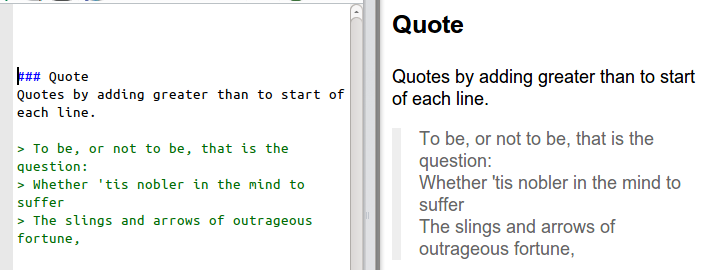
\includegraphics[width=4in]{figures/quote.png}

\end{frame}

\begin{frame}\frametitle{Tables}

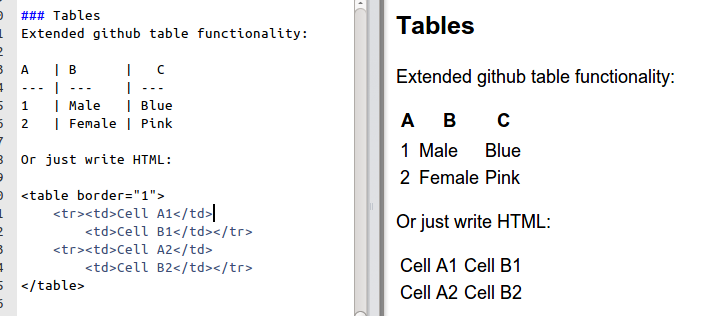
\includegraphics[width=4in]{figures/tables.png}

\end{frame}

\begin{frame}\frametitle{Raw HTML}

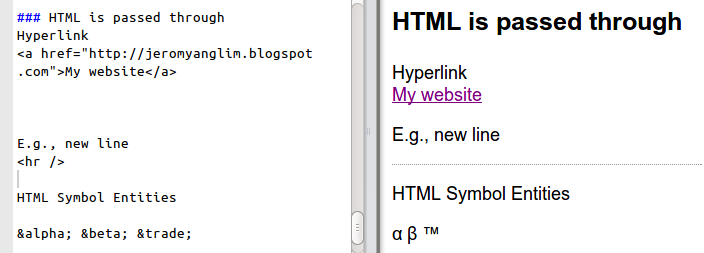
\includegraphics[width=4in]{figures/html.png}

\end{frame}

\section{knitr and R Markdown}

\begin{frame}[fragile]\frametitle{Benefits of knitr}

\begin{itemize}
\item
  knitr supports many markups: LaTeX, Markdown, HTML, reStructuredText
\item
  knitr has really nice defaults
\item
  Simplified figure production

  \begin{itemize}
  \item
    automatically print ggplot2 and lattice figures
  \item
    print figures by default
  \item
    permit interspersing of figures and console output
  \end{itemize}
\item
  Greater extensibility:

  \begin{itemize}
  \item
    output options
  \item
    supports languages other than R
  \end{itemize}
\item
  Simplified caching
\item
  And more: \url{http://yihui.name/slides/2012-knitr-RStudio.html}
\end{itemize}

\end{frame}

\begin{frame}\frametitle{Rstudio}

\begin{itemize}
\item
  Benefits of Rstudio as IDE for R

  \begin{itemize}
  \item
    Open source
  \item
    Works on Linux, Mac, and Windows
  \item
    Many useful features
  \item
    It just works
  \item
    Tight integration with knitr
  \end{itemize}
\item
  But many other options

  \begin{itemize}
  \item
    Emacs with ESS
  \item
    Vim with R plugin
  \item
    Eclipse with StatET
  \item
    etc.
  \end{itemize}
\end{itemize}

\end{frame}

\begin{frame}\frametitle{Rstudio screenshot}

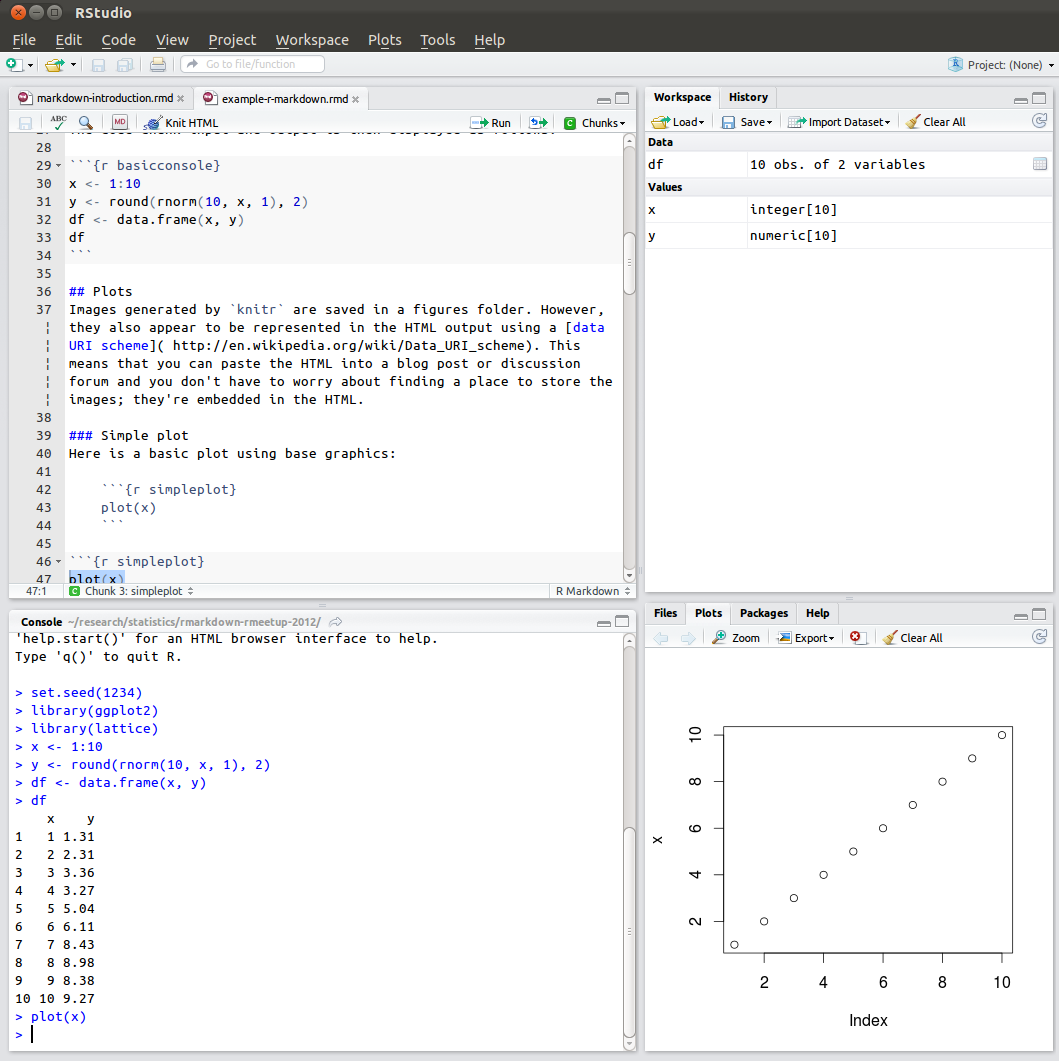
\includegraphics[width=3in]{figures/rstudio-screenshot.png}

\end{frame}

\begin{frame}\frametitle{R Code chunks}

Global options:

\end{frame}

\begin{frame}[fragile]\frametitle{Installation}

\begin{itemize}
\item
  Install Rstudio
\item
  Install knitr \texttt{install.packages("knitr")}
\end{itemize}

\end{frame}

\begin{frame}[fragile]\frametitle{Inline R Code}

\begin{itemize}
\item
  \textbackslash{}texttt\{`r 2 + 2` becomes `4` which becomes 4.
\item
  \texttt{r I(2+2)}
\item
  Markdown \texttt{4} 4 HTML 4 4
\end{itemize}

\end{frame}

\begin{frame}\frametitle{Figures}

\end{frame}

\begin{frame}[fragile]\frametitle{Tables}

\begin{itemize}
\item
  Many options for creating HTML Tables:

  \begin{itemize}
  \item
    R packages: \texttt{xtable}, \texttt{googleVis}, \texttt{R2HTML},
    \texttt{hwriter}
  \item
    markdown extentions: github, pandoc
  \item
    Custom R code
  \end{itemize}
\item
  \texttt{xtable} is a reasonable option
\item
  For informal reports just use console output
\item
  css can be added later to control table appearance
\end{itemize}

\end{frame}

\begin{frame}[fragile]\frametitle{\texttt{xtable} example}

\begin{verbatim}
print(xtable(my_data_frame, caption = "My Caption", 
    digits = 3), type = "html", 
    caption.placement = "top", 
    html.table.attributes = 
    "style=\"border: 1px solid black;\"")
\end{verbatim}

\centerline{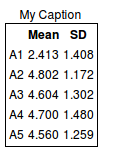
\includegraphics[height=1.5in]{figures/simple_table.png}}

\end{frame}

\begin{frame}\frametitle{Rstudio}

\end{frame}

\begin{frame}[fragile]\frametitle{Caching}

Basic workflow:

\begin{itemize}
\item
  If knitting is quick, don't cache.
\item
  If knitting takes more than ten seconds add
  \texttt{\`}\texttt{r opts\_chunk\$set(cache=TRUE)}\texttt{\`} to the
  top of R Markdown file.
\item
  If caching is causing problems, delete contents of \texttt{cache}
  folder,
\item
  But if caching is causing problems and knitting takes a long time,
  name R code chunks and use the \texttt{dependson} option in knitr (see
  http://yihui.name/knitr/options). Naming also permits selective
  deletion of named R code chunks in the cache directory.
\end{itemize}

\end{frame}

\begin{frame}\frametitle{R package: \texttt{markdown}}

\begin{itemize}
\item
  Devloped by Jeffrey Horner
\item
  R Package that creates more options for converting Markdown to HTML
\end{itemize}

\end{frame}

\begin{frame}[fragile]\frametitle{Replicating R Studio}

\begin{verbatim}
require(knitr) # required for knitting from rmd to md
require(markdown) # required for md to html 
knit('test.rmd', 'test.md') # creates md 
markdownToHTML('test.md', 'test.html') # create html
browseURL(paste('file://', 
    file.path(getwd(),'test.html'), 
    sep='')) # open file in browser
\end{verbatim}

see \texttt{?markdownHTMLOptions} for more options. E.g.,

\begin{verbatim}
markdownToHTML('test.md', 'test.html', 
    options='fragment_only')
\end{verbatim}

\end{frame}

\section{LaTeX}

\begin{frame}\frametitle{knitr with LaTeX}

\begin{itemize}
\item
  Sexpr
\item
  Code chunk delimiters
\end{itemize}

\end{frame}

\section{Conclusion}

\begin{frame}\frametitle{Final thoughts}

\end{frame}

\begin{frame}[fragile]\frametitle{Links}

\begin{itemize}
\item
  knitr: \url{http://yihui.name/knitr/}
\item
  R Studio: \url{http://rstudio.org/}
\item
  R Markdown with R Studio:
  \url{http://rstudio.org/docs/authoring/using_markdown}
\item
  Places to ask questions

  \begin{itemize}
  \item
    R on StackOverflow:
    \url{http://stackoverflow.com/questions/tagged/r}
  \item
    LaTeX: \url{http://tex.stackexchange.com/}
  \item
    knitr: \url{https://github.com/yihui/knitr/issues}
  \end{itemize}
\end{itemize}

\end{frame}
